% \begin{itemize}
% \item component-based commissioning model
% \item control components to handle the commissioning of any existing
%   component in any language
% \item goals: programmable, composable, reusable, efficient
% \item composed of:
%   \begin{itemize}
%   \item meta-model
%   \item graphical language
%   \item concrete language
%   \item formal specification (next section)
%   \item formal operational semantics (next section)
%   \end{itemize}
% \item meta-models of assembly and components (add groups)
% \item example Apache/MariaDB with graphical and concrete syntax
% \item simplified explanation of the operational semantics (middleware)
% \item discussion on the goals
% \end{itemize}

%%%%%%%%%%%%%%%%%%%%%%%%%%
\subsection{Principles}

\mad is a component-based coordination model for commissioning
procedures. More precisely, \mad offers a way to model and
coordinate the execution of complex distributed software commissioning
procedures by adapting the software engineering concept of component
model. Usually component models are used to write code of distributed
software in a modular fashion while having guarantees on their
compositions, thus improving separation of concerns between
developers, easing the way to reuse existing pieces of code and
enhancing flexibility and maintainability of codes. However, writing
functional code is quite different from coordinating commissioning
procedures. Because of this, \mad components are quite different from
usual components.
A \mad component is a type containing a set of places that represent
milestones of the commissioning, and a set of transitions that connect
the places together and represent actions to be performed between
milestones (\eg \texttt{apt-get install}, \texttt{docker pull}
etc.). If multiple transitions leave a place, their parallel execution
is automatically handled and synchronized by \mad. A component may
have dependencies to other components. Such dependencies are
declared through an object well-known in component-based software
engineering: ports. Four types of ports, working in pairs, are
available in \mad: service-provide and service-use, data-provide and
data-use ports. By using ports, each component type can be defined
independently and component instances can be connected later by
another developer, thus improving the separation of concerns and the
reuse of commissioning procedures. \mad components are called \emph{control}
components as they only intend to model the commissioning procedure of
an already existing piece of code (component, module or service etc.)
of a distributed software system.

\MC[Hélène, Dimitri]{``piece of code'' -> est-ce qu'on ne parle que de code ou aussi de
ressources ?}

The overall commissioning procedure of a distributed software system
is built by composition in an \emph{assembly}, where component
types are instanciated and connected. All control components execute
simultaneously, thus introducing more parallelism (in addition to
parallel transitions). Intuitively, two components connected by their
respective compatible ports will be automatically coordinated such
that a component cannot use a service or a data if the associated
provide port is not enabled.

\emph{As a result, \mad offers the expressivity to get composable,
reusable and efficient commissioning procedures for complex
distributed software systems.}

\begin{figure}[tbp]
  \begin{center}
    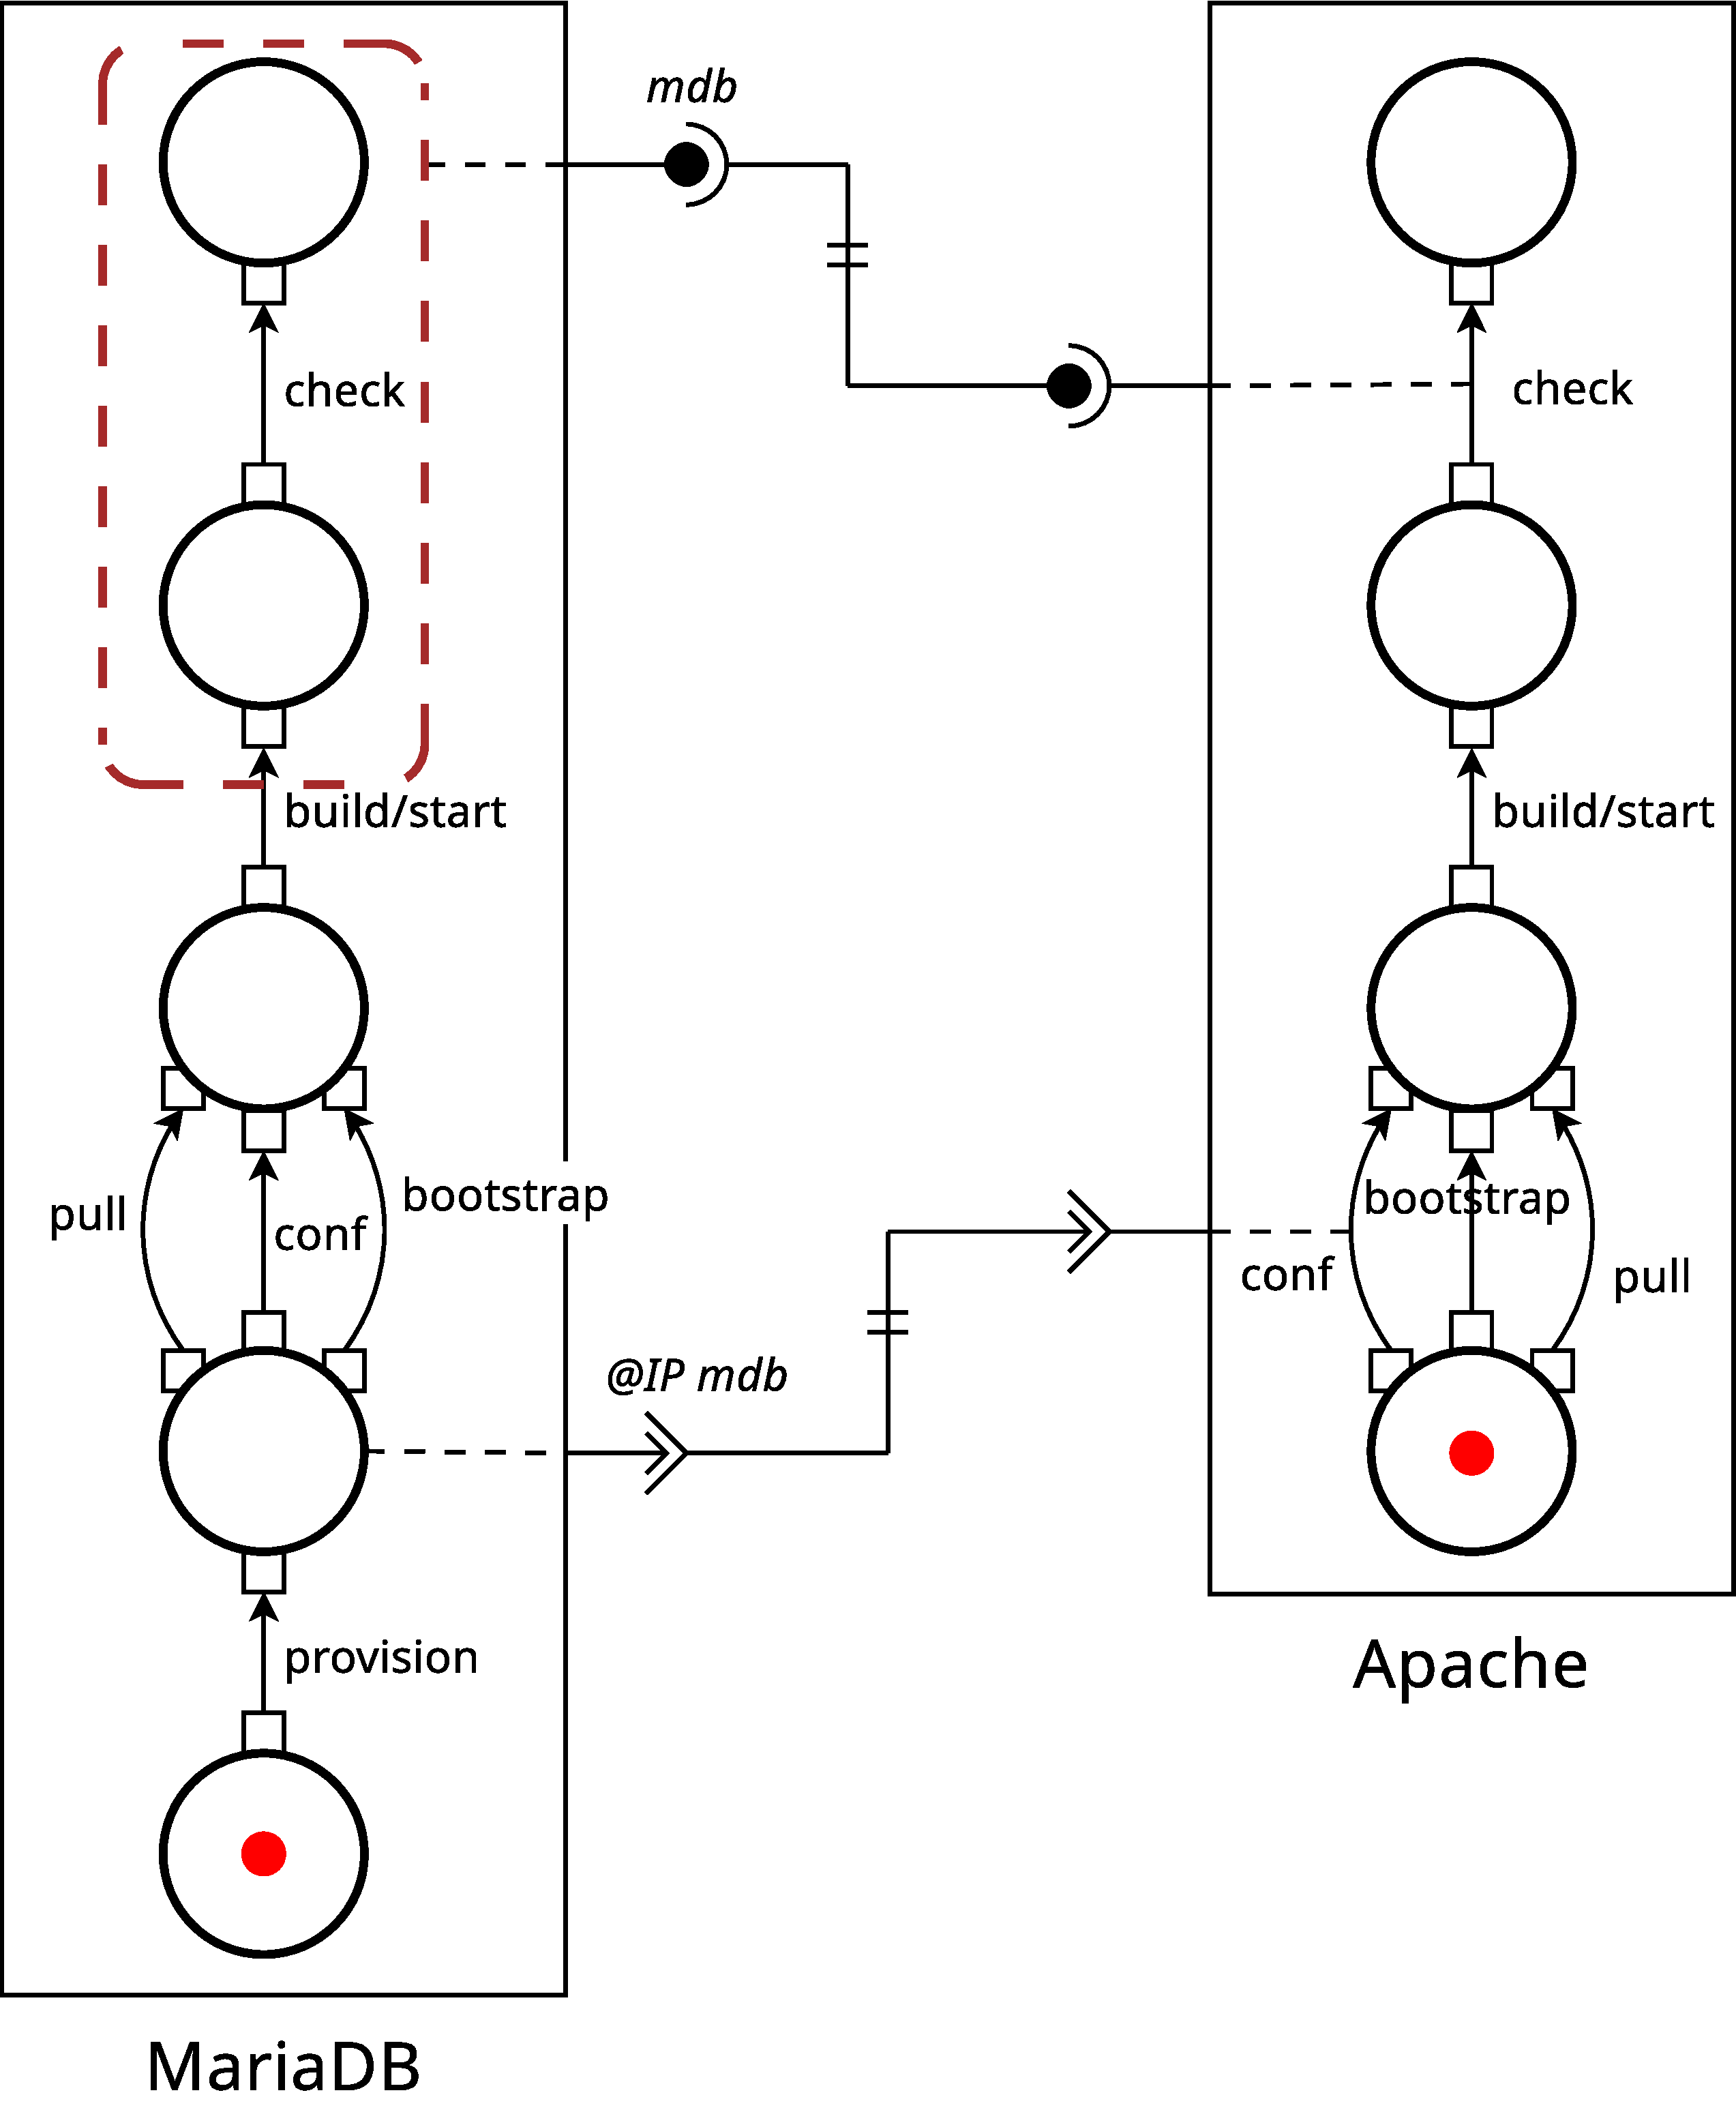
\includegraphics[width=0.7\linewidth]{./images/apachebdd.pdf}
  \end{center}
  \caption{Example of a commissioning assembly with two components
    Apache and MariaDB. Places are represented by circles, transitions
    by arrows between places, service ports by small black circles and
    semi-circles, data ports by outgoing or incoming arrows from
    components. Two initial red tokens are placed in each initial
    place of components in this example.}
  \label{fig:example}
\end{figure}

\MC[Maverick]{TODO: mettre à jour la figure (inverser le nombre de places des composants)}

\paragraph{Example}{ Figure~\ref{fig:example} depicts the \mad
  commissioning of an Apache web server and a MariaDB database. This
  example is based on a real container-based deployment described by
  RedHat\footnote{\url{https://access.redhat.com/documentation/en-us/red_hat_enterprise_linux_atomic_host/7/html/getting_started_with_containers/install_and_deploy_an_apache_web_server_container}}%
  $^,$%
  \footnote{\url{https://access.redhat.com/documentation/en-us/red_hat_enterprise_linux_atomic_host/7/html/getting_started_with_containers/install_and_deploy_a_mariadb_container}}. Two
  \mad component types are declared in this example: Apache
  and MariaDB. Apache contains four places, or millestones, while
  MariaDB contains five places. Some parallel transitions are declared
  for each of the component and can be observed in the figure. Both
  components have two ports. MariaDB provides both a data and a
  service (once installed), while Apache uses a service and a
  data. Figure~\ref{fig:example} shows the assembly of one Apache and
  one MariaDB instanciated from their component types. These instances
  are connected by their ports. Indeed, the Apache configuration need
  the IP adress of the MariaDB component, and the testing phase for
  Apache, called \texttt{check}, uses the MariaDB service.}

In \mad two kinds of \emph{actors} are considered. First, the
developer of a control component, called \emph{dev-comp}, who may be
the author of the associated existing piece of code, or
another developer, or even a system operator or administrator. Second,
the developer of an assembly, called \emph{dev-ass}, who is typically
\HC[All]{le nom me fait rire :D} a system operator or administrator
who wants to write the overall commissioning procedure of a
distributed software system to deploy on their infrastructure. One
important benefit of \mad compared to other approaches is its clear
separation of concerns between the commissioning of a single component
on the one hand and the composition of an assembly, without having to
care aboutthe detailed commissioning of each component on the other hand.
Even if Ansible, Puppet and
Chef, for instance, offer properties close to composition (\eg roles,
playbooks, recipes etc.), the system operator still has to handle the
correct order of composition. Conversely, the correct coordination,
thus the correct order of execution, is automatically guaranteed by
\mad by the composition of the component instances. The composition
viewpoint is illustrated in Figure~\ref{fig:simple} where
\emph{dev-ass} does not need to know the details of each component to
compose them. Such property has also been offered by Aeolus~\cite{}
but without parallelism within components.

\begin{figure}[tbp]
  \begin{center}
    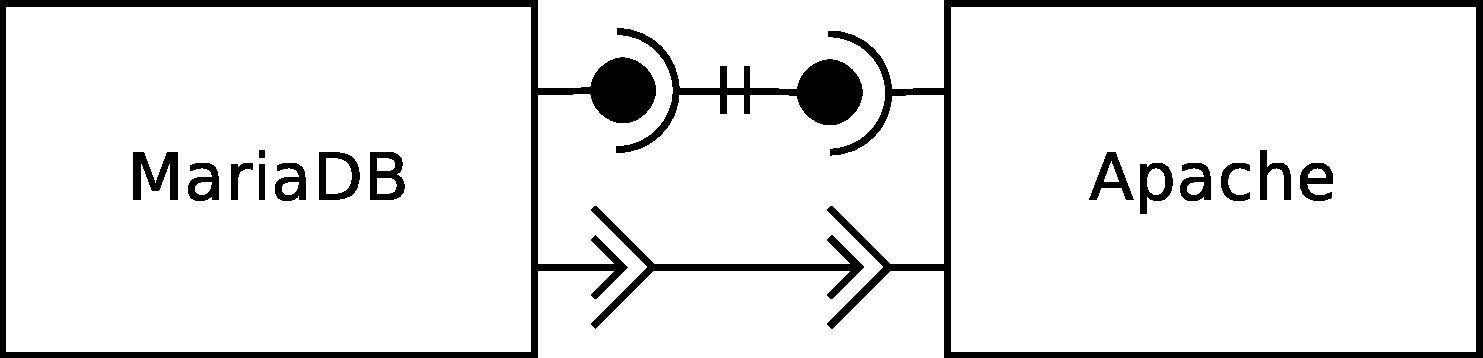
\includegraphics[width=0.6\linewidth]{./images/simpleass.pdf}
  \end{center}
  \caption{\mad assembly of an Apache component and a MariaDB
    component without knowing the details of each component.}
  \label{fig:simple}
\end{figure}

\MC[All]{Nommer chaque élément qui compose \mad ? (langage graphique, language concret, implem, autre ?)}
\mad is a language to model distributed software commissionings.
Second, \mad is a
\emph{graphical language}, as illustrated in Figure~\ref{fig:example},
that can be used to observe and understand how a distributed software
commissioning is modeled, but also to be able to monitor the state of
this procedure. Third, \mad also comes with a \emph{concrete
  language}, which is for now prototyped in Python. Finally, \mad is
able to execute an assembly by following a formal \emph{operational
  semantics}. In this sub-section we give an overview of the
meta-model, the concrete language and the execution semantics of
\mad by using the example of Figure~\ref{fig:example}. Later
Sections~\ref{sec:forma_model} and~\ref{sec:perf_model} will present
the formalization of \mad and its operational semantics, as well as
its theoretical performance model.

%%%%%%%%%%%%%%%%%%%%%%%%%%
\subsection{Meta-model}

\HC[Maverick]{figures a refaire avec nos discussions}

\begin{figure}[tbp]
  \begin{center}
    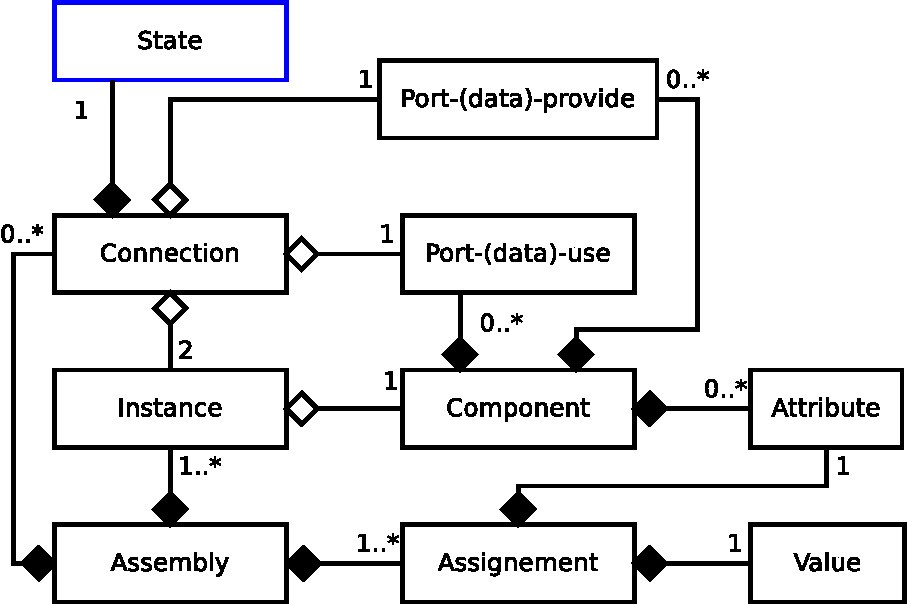
\includegraphics[width=0.9\linewidth]{./images/ass_uml.pdf}
  \end{center}
  \caption{\mad meta-model of an assembly, \ie an overall
    commissioning procedure of a distributed software.}
  \label{fig:mmass}
\end{figure}

Figures~\ref{fig:mmass} and~\ref{fig:mmcomp} respectively depict the
UML diagram representing the \mad meta-model of an assembly, and the
meta-model of a component. A \mad assembly is not different from a
usual assembly in any component model of the literature. An assembly
basically contains component instances, connected to each other
through their compatible ports. One specificity is that \mad handles
four types of ports instead of usually two, by dissociating service
ports from data ports, each having their own semantics. Intuitively,
unlike service ports, data ports act as data registries thus, once
activated, they will remain active forever.

\begin{figure}[tbp]
  \begin{center}
    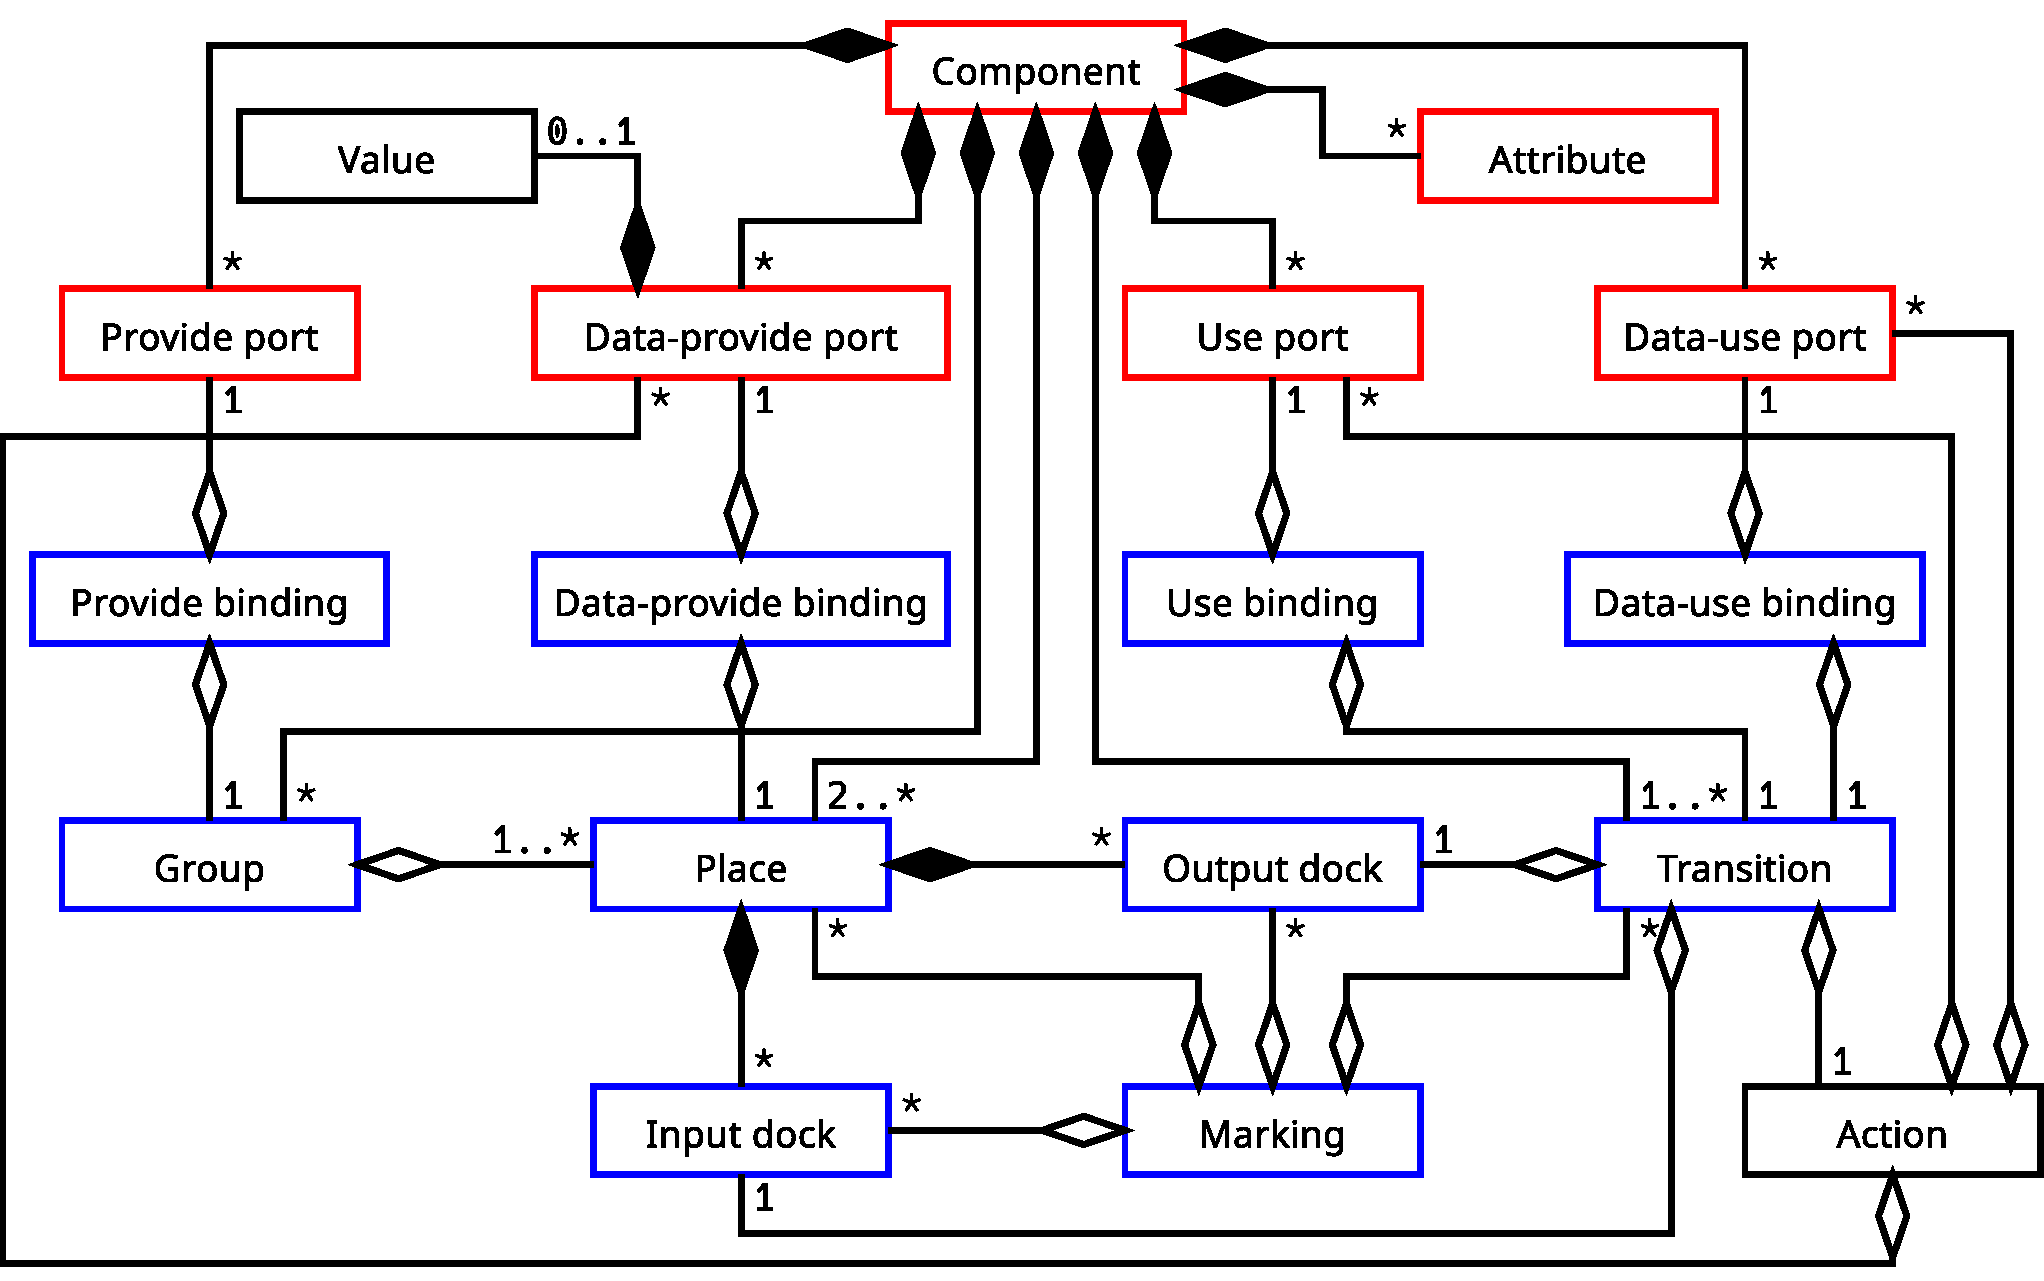
\includegraphics[width=0.9\linewidth]{./images/component_uml.pdf}
  \end{center}
  \caption{\mad meta-model of a component, \ie the commissioning
    procedure of a single component (\ie module or service).}
  \label{fig:mmcomp}
\end{figure}

However, as already explained a \mad component is very different
from usual components in the literature. A component type contains a
set of places, a set of transitions, and a set of service-provide,
service-use, data-provide and data-user ports.
%Each place contains
%input and output docks. A transition is composed of a source and a
%destination dock (from one place to another). Docks are used in the
%formal model to properly handle parallelism and
%synchronizations.
Service-provide ports (service or data) are bound to groups of
places. Those groups of places represent the sub-part of the
commissioning procedures where a given service is provided. A
data-provide port is simply bound to one place from which the data is
provided. Use ports (data or service) are bound to transitions where
the corresponding data or services modeled by ports are actually used
by the code executed by the transition.

%%%%%%%%%%%%%%%%%%%%%%%%%%
\subsection{Concreto language}

\MC[All]{Est-ce qu'on donne un nom à ``Concerto language'' ?}

The concrete syntax of \mad has been implemented in Python. \mad
is a simple declarative language that follows the meta-model
previously detailed to define, first, component types, and second,
assemblies of components. Listing~\ref{codemdb} shows the declaration
of the MariaDB component type of Figure~\ref{fig:example}. Lines 3 to
8 consist in the declaration of the places of the component type. A
place is identified by a unique \texttt{string}. Lines 9 to 15 consist
in the declaration of the transitions of the component type. A
transition is identified by a unique key (a \texttt{string}), and is
associated through a dictionnary to a source and a destination
place. Moreover, each transition is associated to a function to call
to perform associated actions. For instance, the function
\texttt{f\_pull} of transition \texttt{pull} is declared line 20 and
will contain the code to execute during this transition. Finally lines
16 to 19 declare the ports of the component type. A port is identified
by a unique key (a \texttt{string}), and is associated to a type and
the elements to which it is bound. As already described,
service-provide ports are bound to a set of places, data-provide ports
to a single place, and both service-use and data-use ports to a set of
transitions. In the case of MariaDB one service-provide port, namely
\texttt{serv}, is provided both at \texttt{std} and \texttt{chd}
places, and one data-rpovide port, namely \texttt{ip} is provided from
the first place \texttt{wtg}.

\begin{lstlisting}[label=codemdb,caption=Madeus code of the MariaDB
  component type.]
class MariaDB (Component):
  def create(self):
    places = [
        'wtg',
        'cfd',
        'std',
        'chd'
    ]
    transitions = {
        'pull': ('wtg', 'cfd', self.f_pull),
        'conf': ('wtg', 'cfd', self.f_conf),
        'bootstrap': ('wtg', 'cfd', self.f_boots),
        'start': ('cfd', 'std', self.f_start),
        'check': ('std', 'chd', self.f_check)
    }
    dependencies = {
        'ip': (DepType.DATA_PROVIDE, 'wtg'),
        'serv': (DepType.PROVIDE, ['std','chd'])
    }
    def f_pull(self):
        # execution of bash scripts
        # execution of ansible playbooks
        # etc.
    def f_conf(self):
        # ...
    def f_boots(self):
        # ...
    def f_start(self):
        # ...
    def f_check(self):
        # ...
\end{lstlisting}


Similarly, the Listing~\ref{codeapache} shows the decalaration of the
Apache component type of Figure~\ref{fig:example} which has one more place
and one more transition compared to MariaDB. Furthermore, the Apache
component type contains one service-use port and one data-use port
(lines 18 to 21).

\begin{lstlisting}[label=codeapache,caption=Madeus code of the Apache
  component type.]
class Apache (Component):
  def create(self):
    places = [
        'wtg',
        'prd',
        'cfd',
        'std',
        'chd'
    ]
    transitions = {
        'provision': ('wtg','prd', self.f_prov),
        'pull': ('pr', 'cfd', self.f_pull),
        'conf': ('pr', 'cfd', self.f_conf),
        'bootstrap': ('prd', 'cfd', self.f_boots),
        'start': ('cfd', 'std', self.f_start),
        'check': ('std', 'chd', self.f_check)
    }
    dependencies = {
        'ipMDB': (DepType.DATA_USE, ['conf']),
        'serviceMDB': (DepType.USE, ['check'])
    }

    def f_prov(self):
        # execution of bash scripts
        # execution of ansible playbooks
        # etc.
    def f_pull(self):
        # ...
    def f_conf(self):
        # ...
    def f_boots(self):
        # ...
    def f_start(self):
        # ...
    def f_check(self):
        # ...
\end{lstlisting}


Finally, the Listing~\ref{codeass} shows the decalaration of the
assembly of components of Figure~\ref{fig:example}. First, lines 6 and
7 respectively instanciate component types MariaDB and Apache
previously declared. Second, line 9 to 13 are as follows: the creation
of an assembly, the addition of component instances to the assembly,
the connections of the components. Finally, lines 15 and 16 run the
assembly to perform the commissioning of MariaDB/Apache. An overview
of this execution is given in the next section.

\begin{lstlisting}[label=codeass,caption=Madeus code of the assembly
  of Figure~\ref{fig:example}.]
import mariadb
import apache

if __name__ == '__main__':

  mdb = MariaDB() # Component B
  apache = Apache() # Component C

  ass = Assembly()
  ass.add('MDB', mdb)
  ass.add('Apache', apache)
  ass.connect(apache, 'ipMDB', mdb, 'ip')
  ass.connect(apache, 'servMDB', mdb, 'serv')

  mad = Mad(ass)
  mad.run()
\end{lstlisting}


%%%%%%%%%%%%%%%%%%%%%%%%%%
\subsection{Execution}

In \mad, executing a commissioning procedure requires to execute an
assembly. \HC[Helene, Maverick]{TODO introduire la notion de token}
The \mad execution model is governed by operational semantics rules to
move tokens from places to transitions within components. Those rules
are inspired from Petri nets rules but \mad places and transitions
are different from Petri nets places and transitions, and additional
elements such as groups or ports also make \mad different from
Petri nets. Details of the transformation from a \mad assembly to a
Petri net have been given in~\cite{}. The execution of a \mad assemvly
is defined by seven operational semantics rules. In this section we only
sketch the role of each of these rules which are formally specified in
Section~\ref{sec:forma_model}. Before giving the role of each rule,
one can note in Figure~\ref{fig:example} the small squares that
have not been explained yet. These squares respresent \emph{docks}. Each
place has input and output transitions, and each transition has a
source dock and a destination dock. Docks have not been detailed
previously because they are automatically infered from the concrete
syntax of \mad. Though, this concept is needed to explain the
execution of a \mad assembly as it is used to handle parallelism and
synchronization of transitions.
%
\begin{enumerate}
\item \emph{Firing a transition}: when the source dock of a transition
  contains a token and when all use ports of a transition have their
  associated connections activated, the token is moved from the source
  dock to the transition, which is not considered atomic as it is
  associated to an action function.
\item \emph{Ending a transition}: when a transition holds a token and
  when the action associated to the transition is terminated, the
  token is moved from the transition to its destination dock.
\item \emph{Joining a place}: when all input docks associated to a
  place hold a token, tokens can be merged to a single one placed
  within the place.
\MC[Hélène]{Joining -> Entering a place?}
\item \emph{Leaving a place}: when a place holds a token, and if the
  token leaving that place does not cause a provide port currently
  used by other components to be disabled,
  the token can be duplicated and placed in each output dock of the
  place.
\item \emph{Enabling use-provide connection}: a use-provide connection
  which is disabled can be enabled when the group associated to the
  provide port holds a token.
\item \emph{Disabling use-provide connection}: a use-provide
  connection which is enabled becomes disabled as soon as there is no
  more token in any group associated to the provide port.
\item \emph{Enabling data connection}: a data-use-provide connection
  which is disabled can be enabled when the place associated to the
  provide port holds a token. In this case the value is taken from one
  of the previous transition actions.
\end{enumerate}

One can note that a data connection cannot be disabled. It
indefinitely holds the last data value.
%\CP[HC]{Correct?}
%\HC{je n'ai pas parlé des groupes pour simplifier le discours. je ne pense pas en parler car ce n'est pas utile dans les exemples.}
%\CP{ok}

\begin{figure}[tbp]
  \begin{center}
    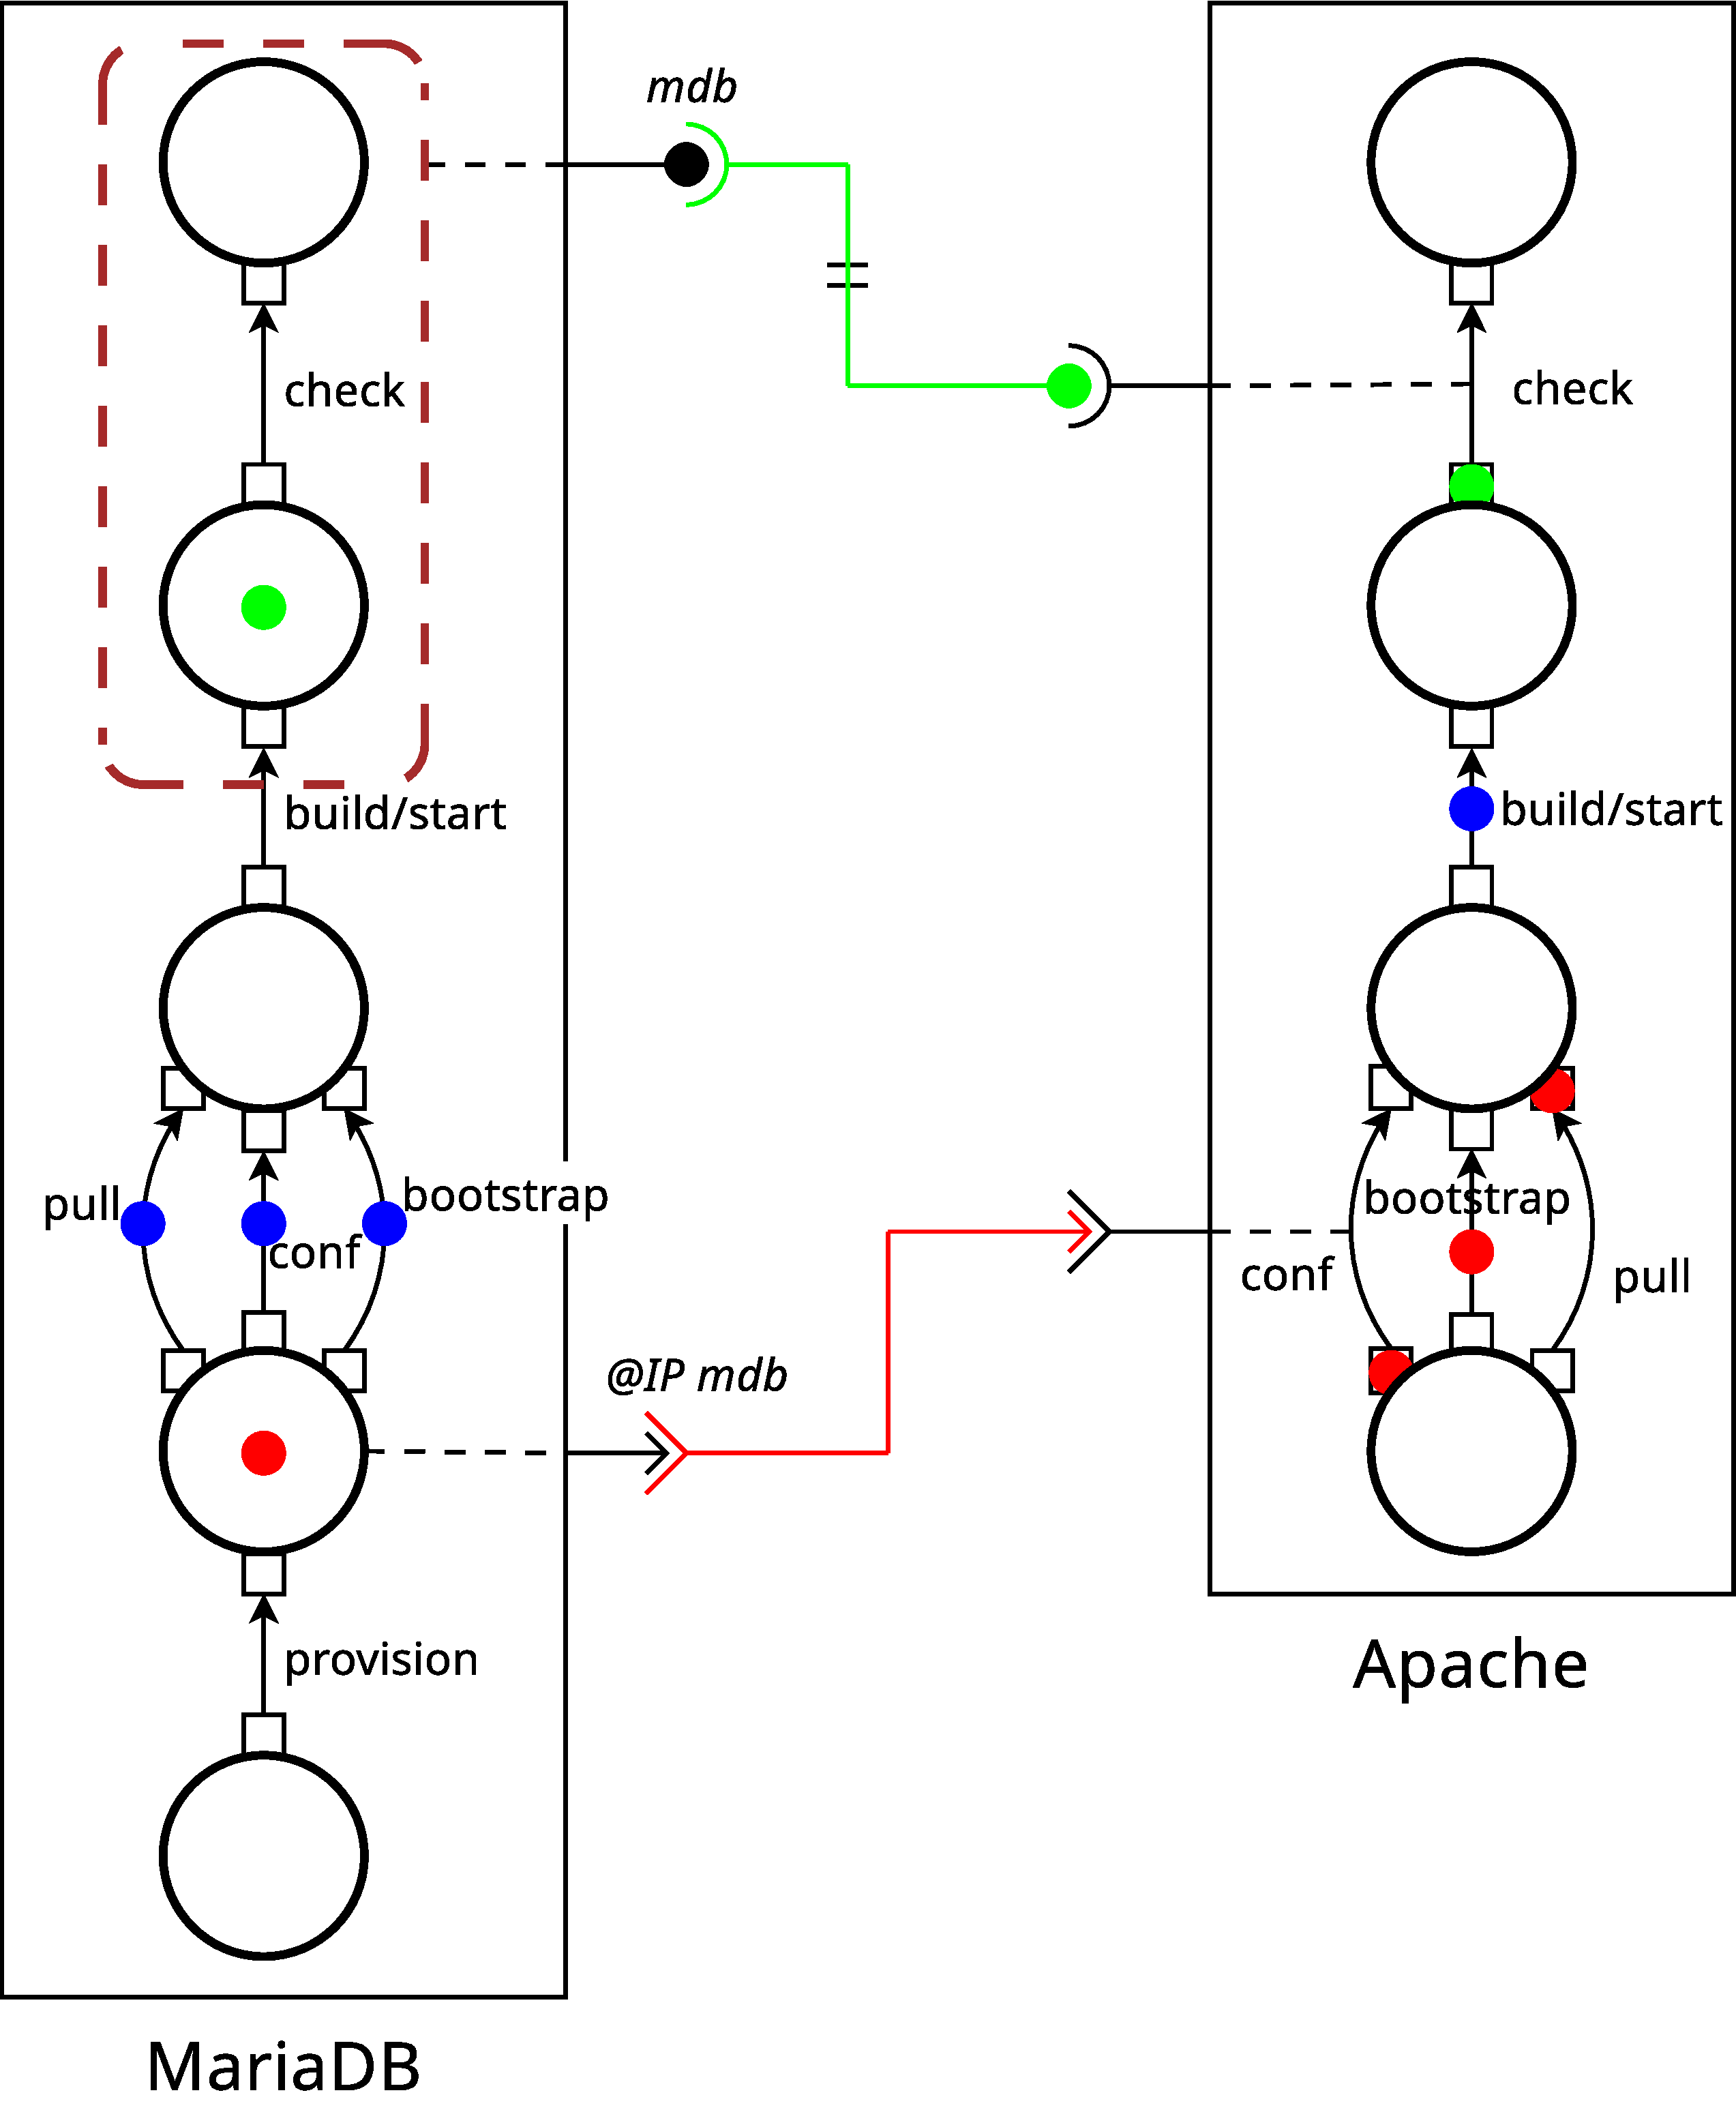
\includegraphics[width=0.7\linewidth]{./images/scenari.pdf}
  \end{center}
  \caption{Three possible intermediate configurations during the commissioning
  of the assembly presented in Figure~\ref{fig:example}. Each configuration is
  represented by a different color.}
  \label{fig:scenari}
\end{figure}

\subsubsection*{Apache/MariaDB Example: \mad Execution}

We discuss now the commissioning of the Apache/MariaDB
example.  The initial assembly, given in Figure~\ref{fig:example}, has
already been described. Figure~\ref{fig:scenari} depicts three example
configurations that may occur at different steps of the commissioning.
The concept of configuration, which is introduced formally in
Section~\ref{sec:forma_model}, intuitively corresponds to a snapshot of
the execution of an assembly (location of the tokens and values
in the data-provide ports). In chronological order, the first
configuration is represented with red tokens, the second one with blue
tokens, and the third one with green tokens.

First, one can note that as MariaDB provides its IP address in its
first place, the associated connection between MariaDB and Apache is
immediately enabled. In the first configuration, the red token of MariaDB
has been able to move from its initial place to its three output
docks. Then, each transition in each branch is able to start as they
are not bound to any port. Simultaneously, the Apache component has
been able to start its \emph{provision} transition and reaches its
parallel branches: \emph{pull} and \emph{conf} can directly start. The
\emph{conf} transition, however, has to wait its associated connection
to be enabled. As the connection has been enabled in the first place
of MariaDB, the red token of the source dock of \emph{conf} can move
to \emph{conf}.

In the second configuration (blue tokens), the MariaDB component has reached
its second place. Both \emph{bootstrap} and \emph{conf} transitions of Apache
have finished but the \emph{pull} transition is still running. For this
reasons the three docks responsible for the join will not release the
tokens until \emph{pull} is terminated. As soon as \emph{pull}
finishes, the three tokens are merged into one token and set to the
next place.%, as MariaDB has already publishes an IP on the data port.

The third configuration illustrates an example where MariaDB reaches
its last place. As soon as this place holds a token, its associated
provide connection is enabled. Finally, the \emph{check}
transition of Apache that is using services of MariaDB is able to
start, once the connection is enabled.
